\chapter{$\mu$GPD}
\label{chap:chapter5}

In the context of X-ray polarimetry, the current Gas Pixel Detectors that are employed on board of IXPE do not match the requirements of the next generation of X-ray polarimeters, such as eXTP. The strictest requirements that have to be satisfied concern the ability to detect photons at a much higher rate than IXPE and to improve the detector stability over time.

The current GPDs employ a finely pixelated ASIC to reconstruct the two-dimensional photoelectron track produced by the absorption of a X-ray photon. This is at the basis of how a photoelectric polarimeter works, and thanks to 50 $\mu$m wide pixels a GPD can perform it with good accuracy, which is translated into a high polarization sensitivity.

As mentioned in Chap. \ref{chap:chapter3}, the main limitations of a GPD are the residual non-uniformities in the azimuthal response, which lead to the so-called spurious modulation, and rate-dependent gain variations. Both these problems can be attributed to the multiplication element of the GPD, the GEM.

The spurious modulation is caused by the manufacturing process of the GEM, where small shape variations between the holes induce a position-dependent systematic effect which is difficult to characterize and correct.

On the other hand, rate-dependent gain variations are attributed to the large dielectric surface inside a GEM hole, which leads to the trapping of part of the charge produced during the avalanche. The consequence of this dielectric charging phenomenon is a change in the configuration of the electric field inside the hole, which results in the decrease of the gain factor.

If the detector is constantly exposed to radiation, charges accumulate with time and the gain keeps varying until a saturation level that depends on the event rate, or more precisely on the incoming energy flux. This means that when switching observations between sources with different fluxes the gain is not stable until a new equilibrium level.

A new type of multiplication stage is under development to replace the GEM and overcome these limitations. The idea behind $\mu$GPD \cite{sgro2026} is to use a micro-gap-like \cite{angelini1993} structure built directly on top of the ASIC.

\section{Detector design}

$mu$GPD represents one of the possible successors of the current GPD generation. The basic working principles remain the same, that is a photoelectric polarimeter which employs a gas active volume to absorb X-ray photons and produce a photoelectron, which is emitted in a direction that depends on the photon polarization. The photoelectron track produced by primary ionization is used to measure the emission angle, and for this purpose the charges are multiplied and subsequently read by an ASIC which acts as collection anode.

The fundamental difference is in the multiplication stage, which in $\mu$GPD consists of structures deposited directly on top of the ASIC. A comparison between the current and one of the proposed designs is shown in Fig. \ref{fig:mugpd}.

The design and the idea behind these structures are similar to micro-gap chambers, which are based on two metal layers separated by a thin isolation layer. The upper-most layer is segmented in one-dimensional or two-dimensional structures only a few $\mu$m large an acts as the anode, while the bottom layer is usually a plane and acts as the catode

Applying a potential difference between the two electrodes generates a strong electric field in a small volume just above the anode. The primary ionizations electrons are drifted toward the anode, where they are accelerating by the electric field and produce an avalanche. The electrons are collected by the anode, while the ions are collected by the bottom layer cathode. An example of the avalanche process is shown in Fig. \ref{fig:avalanche}.

This design is a good candidate to solve the issues of the current generation of GPD. First, the deposition of the dielectric and the anode on top of the ASIC is made with photolitographic techniques, which allow to achieve sub-micron precision in the structure manufacturing. This way, gain non-uniformities across the sensor are strongly reduced. Furthermore, the surface of exposed dielectric is small and the amount of charge that can be accumulated is reduced, improving gain stability.

\begin{figure}[!t]
    \centering
    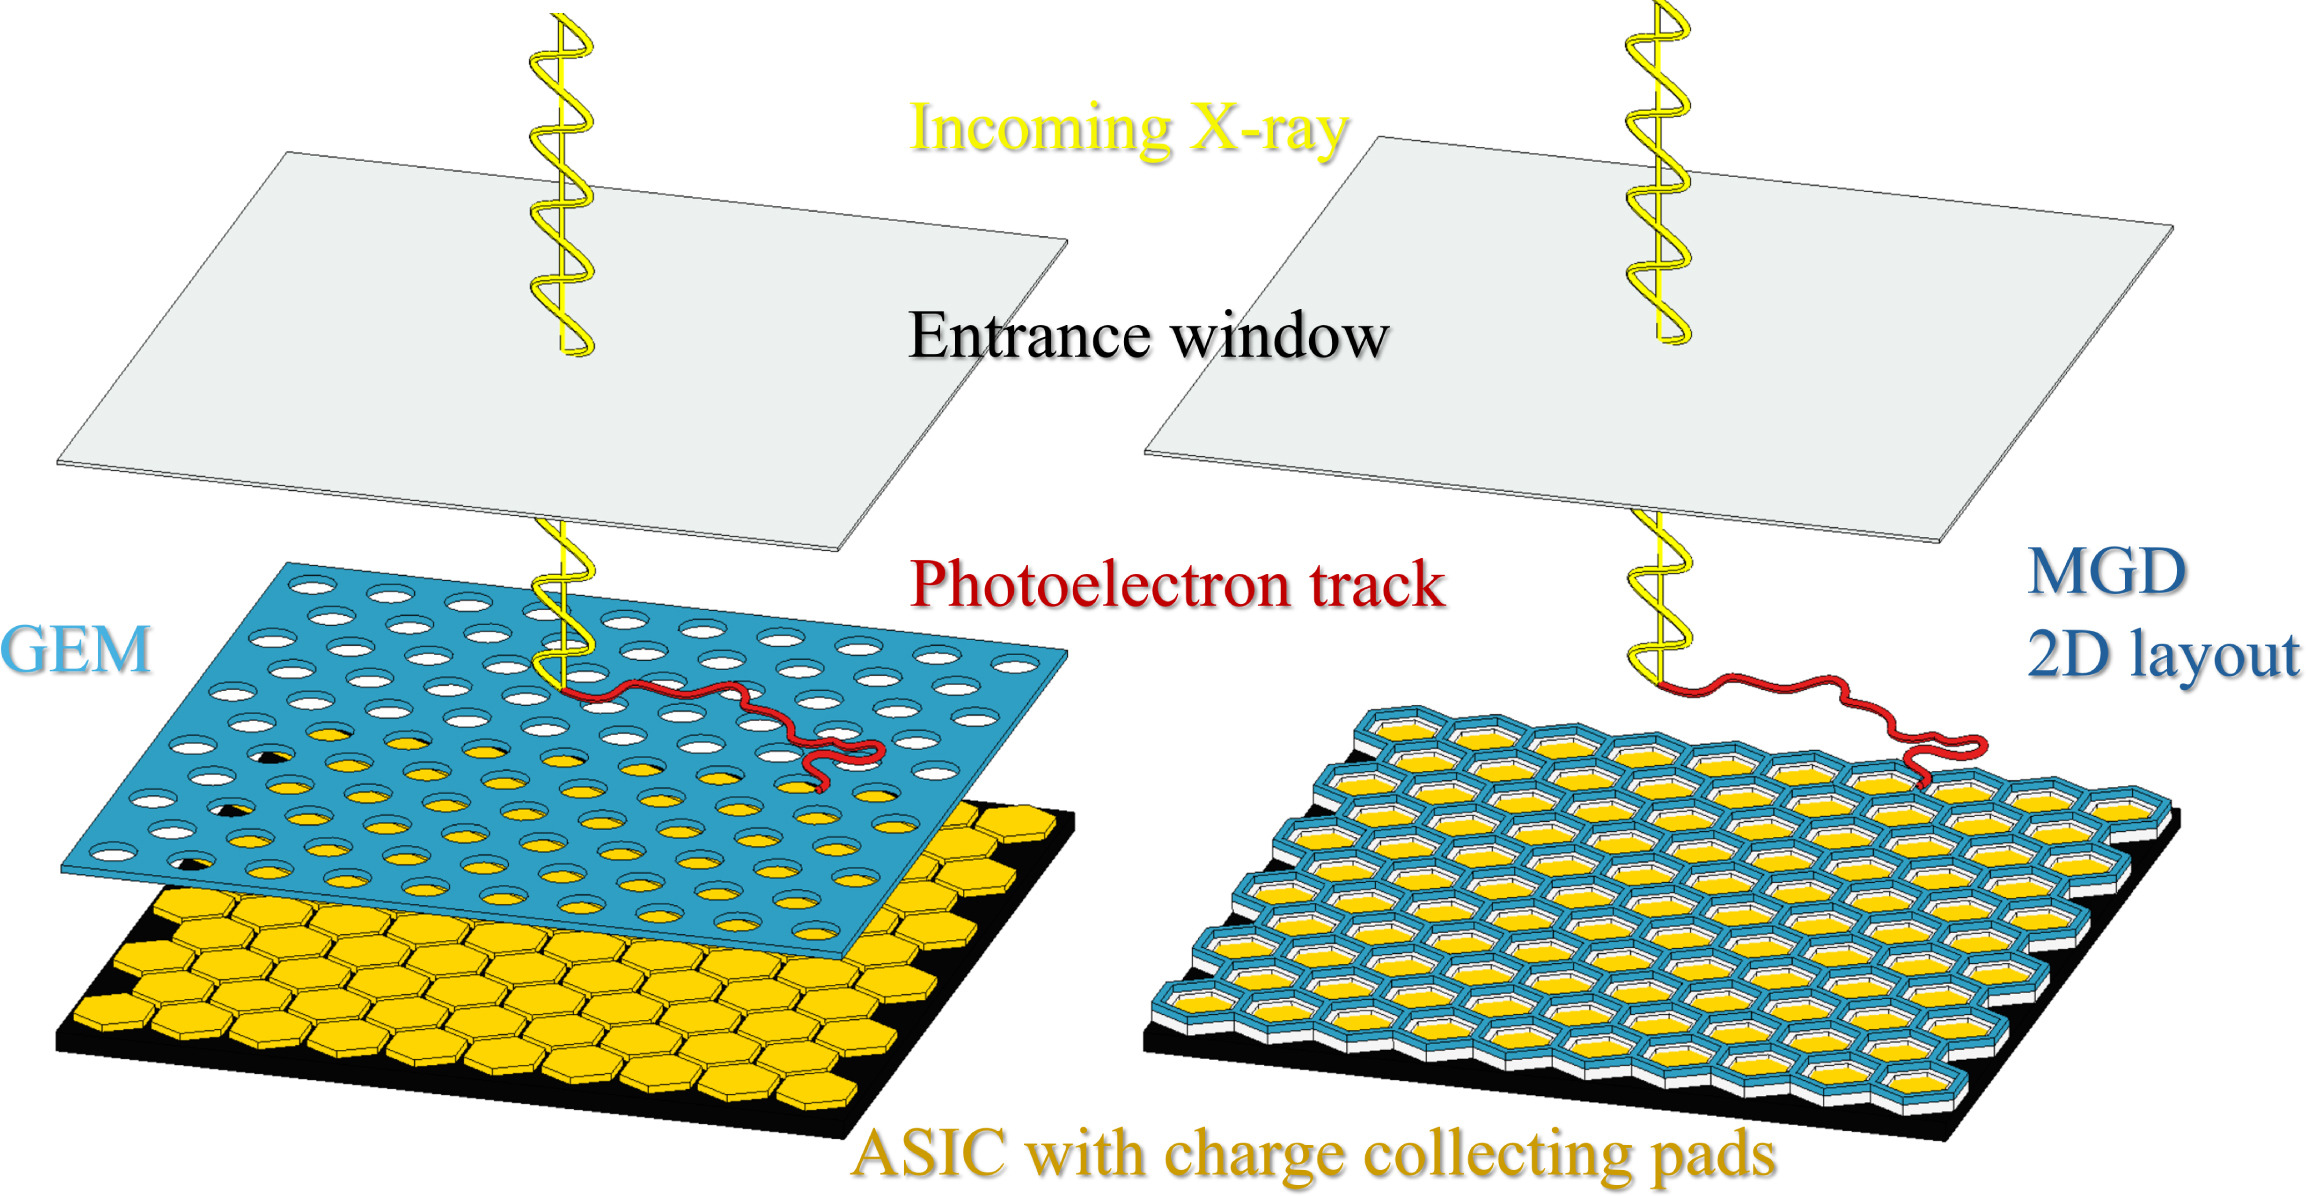
\includegraphics[width=0.7\linewidth]{figures/chapter5/mugpd}
    \caption{Comparison between the current GPD configuration (left panel) and the new proposed configuration with a hexagonal two-dimensional multiplication structure (right). X-rays are absorbed by the active gas volume and emit a photoelectron, which drifts toward the electron multiplier structure. In both cases the track shape is preserved by the multiplication structure. Image taken from \cite{sgro2026}.}
    \label{fig:mugpd}
\end{figure}


\begin{figure}[htpb]
    \centering
    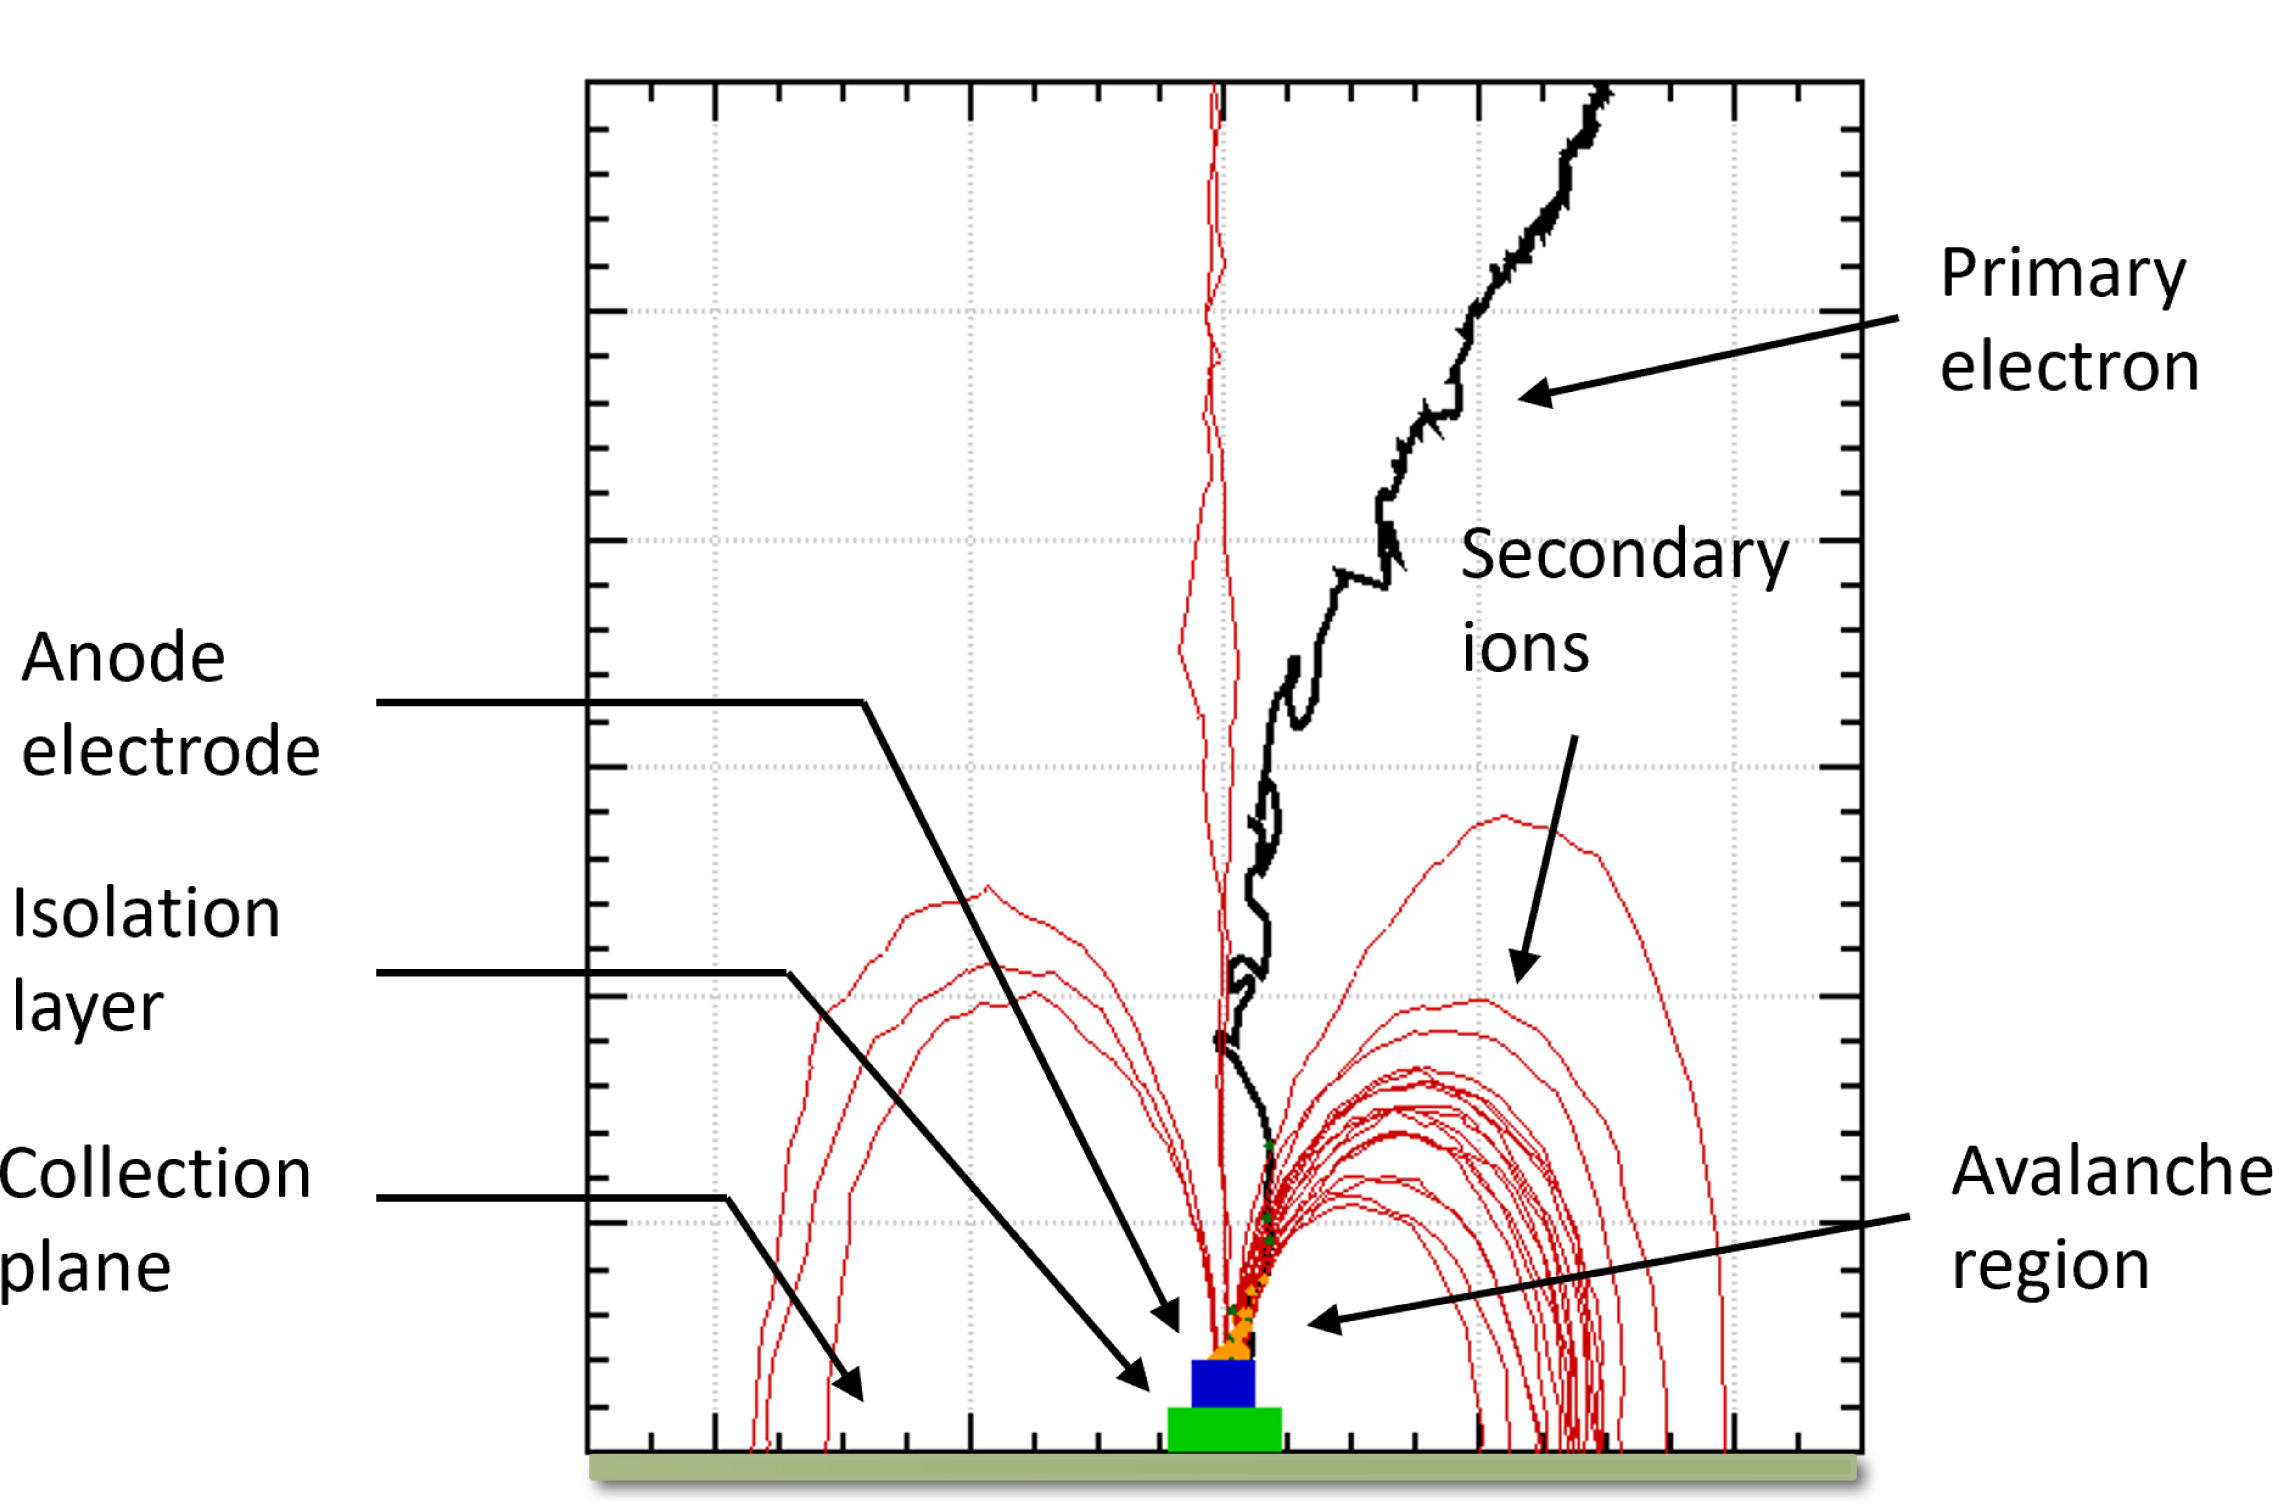
\includegraphics[width=0.6\linewidth]{figures/chapter5/avalanche}
    \caption{Schematic representation of how a micro-gap works. The avalanche is produced due to the strong electric field on top of the anode when a primary ionization electron is drifted toward it. Image taken from \cite{sgro2026}.}
    \label{fig:avalanche}
\end{figure}

At the current prototype stage, multiple anode geometries have been developed to understand which one provides the best detector performances while preserving the two-dimensional nature of the GPD. The proposed geometries are both one-dimensional and two-dimensional structures.

The one-dimensional structures consist of multiple parallel strips that run along  
the pixels. There are different designs currently under study, which vary in pitch and how they are aligned with respect to the pixels. In particular, one design has a pitch of 43.3 $\mu\text{m}$, with a strip aligned to the center of each pixel row. The other two designs have a larger pitch of 86.6 $\mu\text{m}$, where the strips are either aligned to the pixel centers or offset with respect to them.

For the two-dimensional structure the anode has the same shape of the hexagonal pixels, thus each pixel is surrounded by the anode line along its perimeter, as shown in Fig. \ref{fig:mugpd}.

In all the designs the the anode metal is made of aluminum, with a thickness of 2 $\mu$m and 5 $\mu$m wide. The isolation layer below the anode is built with high dielectric strength polyimide 2 $\mu$m thick and 13 $\mu$m wide.


\section{Prototype testing and performances}

At this stage of development, the primary objective is to verify whether these structures can withstand high voltages, which can cause breakdown sparks or leakage currents, and if they can achieve a gain comparable to that of a GEM at a sufficiently low voltage. Another relevant property that can be characterized is the energy resolution that the structures are able to achieve.

Various tests of the anode structures have been performed under different working conditions to verify their feasibility as multiplication stage in the next generation of GPD and to characterize their performances.

\subsection{Implementation on silicon wafer}
The first test that has been performed by building the structures directly on top of a high-resistivity silicon wafer, shown in Fig. \ref{fig:mugpd_wafer}, which acts as the collection layer. This first demonstrator serves to verify the possibility of creating these structures with photolitography processes on top of a substate similar to that of XPOL chips without compromising it.

To test the gain the wafer is placed inside a dedicated gas chamber. The metallic layer of a custom PCB is placed in contact with the back of the wafer to provide negative high voltage, while the anode structures are kept at 0 V.

\begin{figure}[!t]
    \centering
    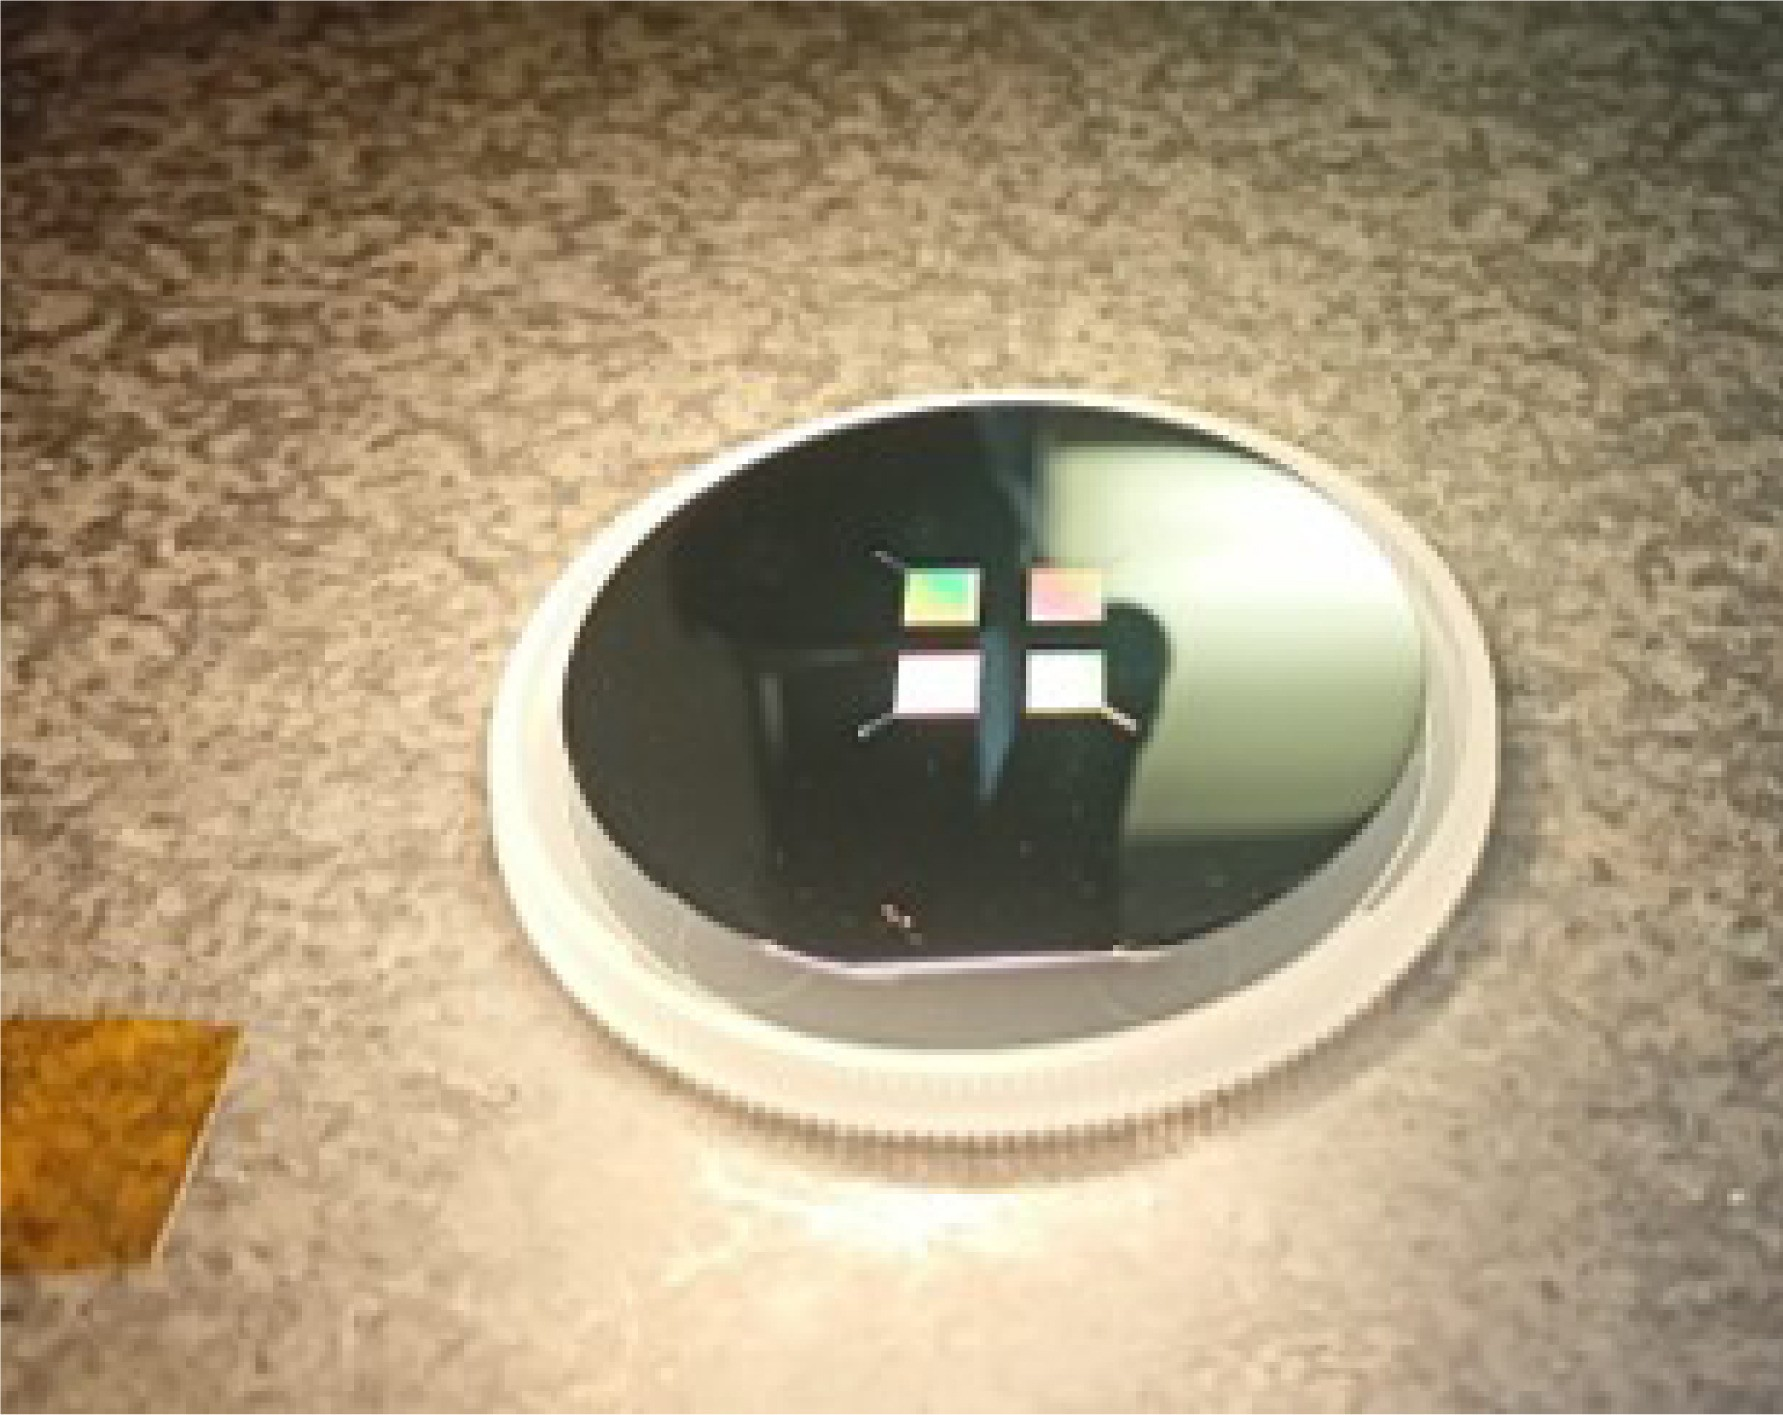
\includegraphics[width=0.6\linewidth]{figures/chapter5/mugpd_wafer}
    \caption{Picture of the silicon wafer with the four anode structures built on top. Image taken from \cite{sgro2026}.}
    \label{fig:wafer_performance}
\end{figure}


The anode structures are connected to a single channel spectroscopic amplifier which in turn is connected to a multichannel analyzer.

To define the absorption and drift region, a 1 cm thick spacer is placed on top of the structures. The entire assembly is placed in a closed box flushed with a mixture of Ar/Isobutane 80/20.

The structures are irradiated with a $^{55}$Fe source placed on top. $^{55}$Fe decays by electronic capture in $^{55}$Mn and it emits fluorescence radiation, with about 90\% probability of emitting $K\alpha$ at 5.9 keV and about 10\% probability of emitting $K\beta$ at 6.5 keV.

The focus of this initial test are the one-dimensional structures, comparing two designs with 43.3 $\mu$m and 86.6 $\mu$m pitch.

Before measuring the gain at different high voltage configurations, the electronic chain is calibrated with a charge injection circuit with a known input capacitance in order to convvert ADC values to charge.

For these preliminary tests the observed spectrum is fitted with a single Gaussian, even though the energy resolution is good enough to observe an asymmetry in the $K\alpha$ emission line due to the presence of the $K\beta$ line. The mean value of the best-fit Gaussian is used to estimate the gain, while the FWHM is used to estimated the energy resolution.

The dependence of gain and energy resolution as a function of the voltage difference of the gap is shown in Fig. \ref{fig:wafer_performance}. For the gain the exponential behaviour described in Eq. \ref{eq:exp_gain} is clearly visible. For both structures a gain of a few hundreds is achievable with voltages below 400 V, of the same magnitude of the GEM gain in GPDs, which is about 200.

It is also possible to observe that in the volateges range under test, energy resolution improves with higher gain. The best energy resolution is achieved by the 86.6 $\mu$m design, which is also the design that can reach a higher gain at lower voltages with respect to the 43.3 $\mu$m design.

\begin{figure}[htpb]
    \centering
    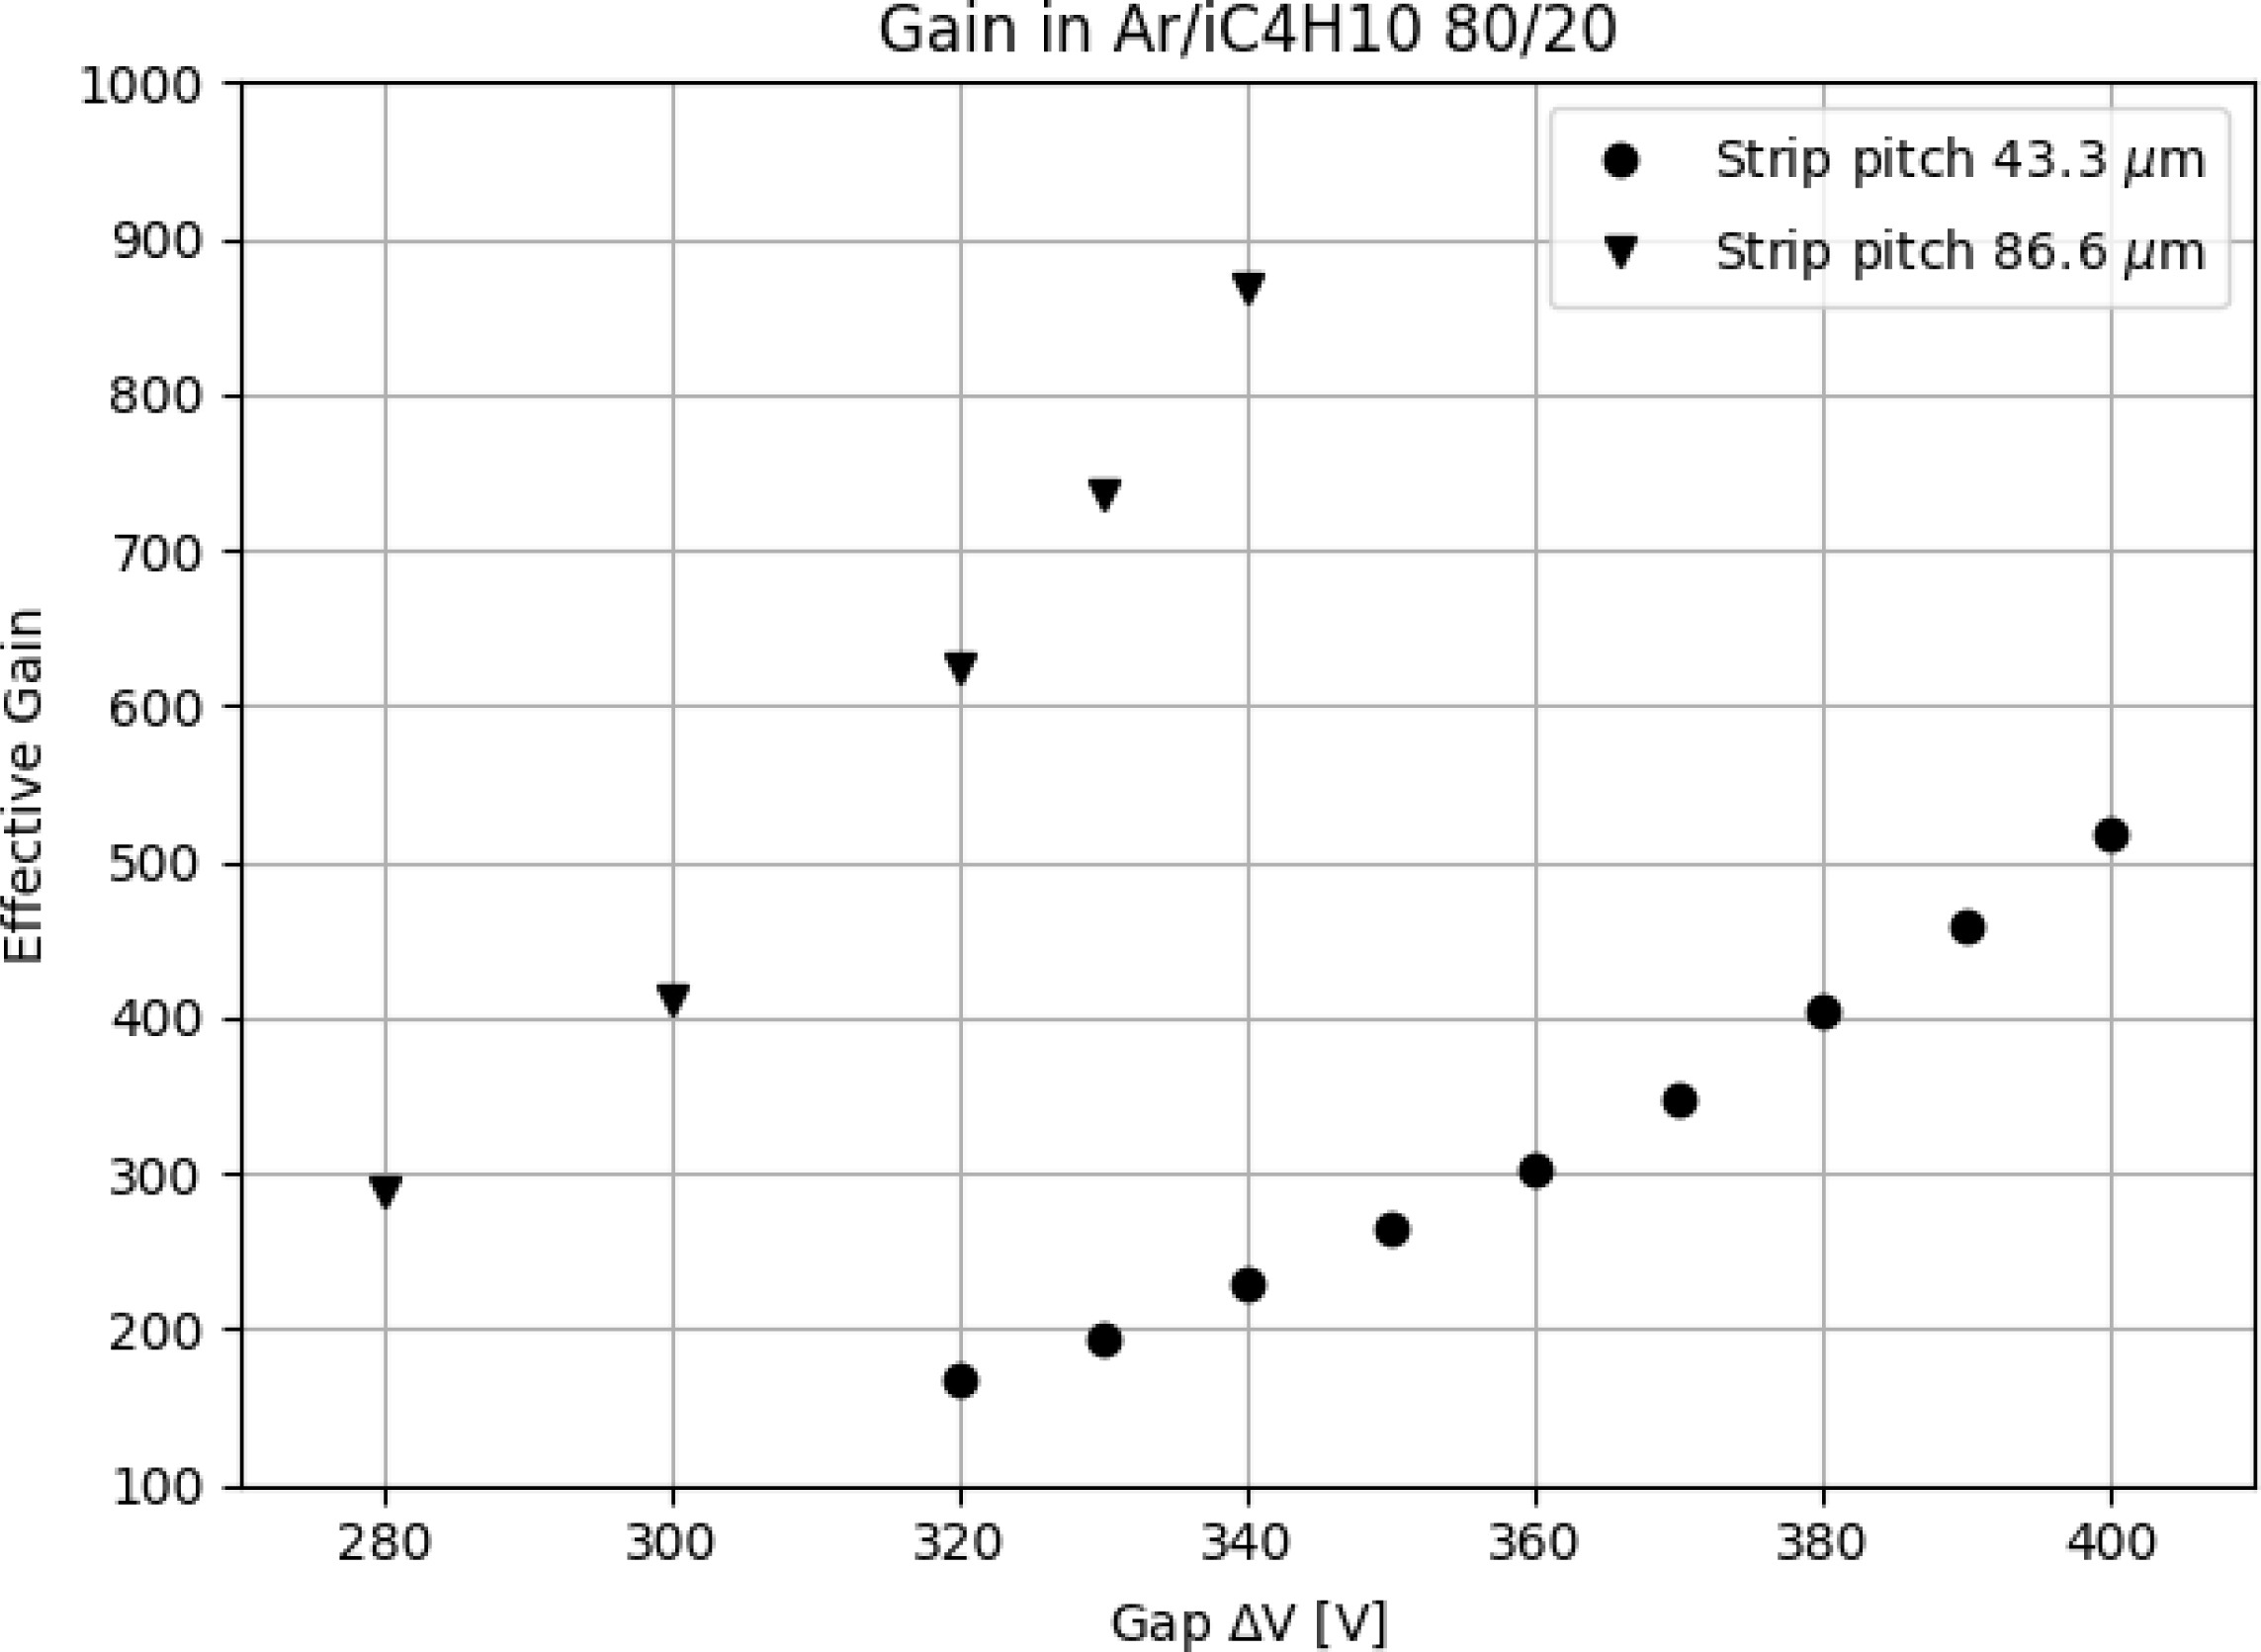
\includegraphics[width=0.49\linewidth]{figures/chapter5/gain_wafer}
        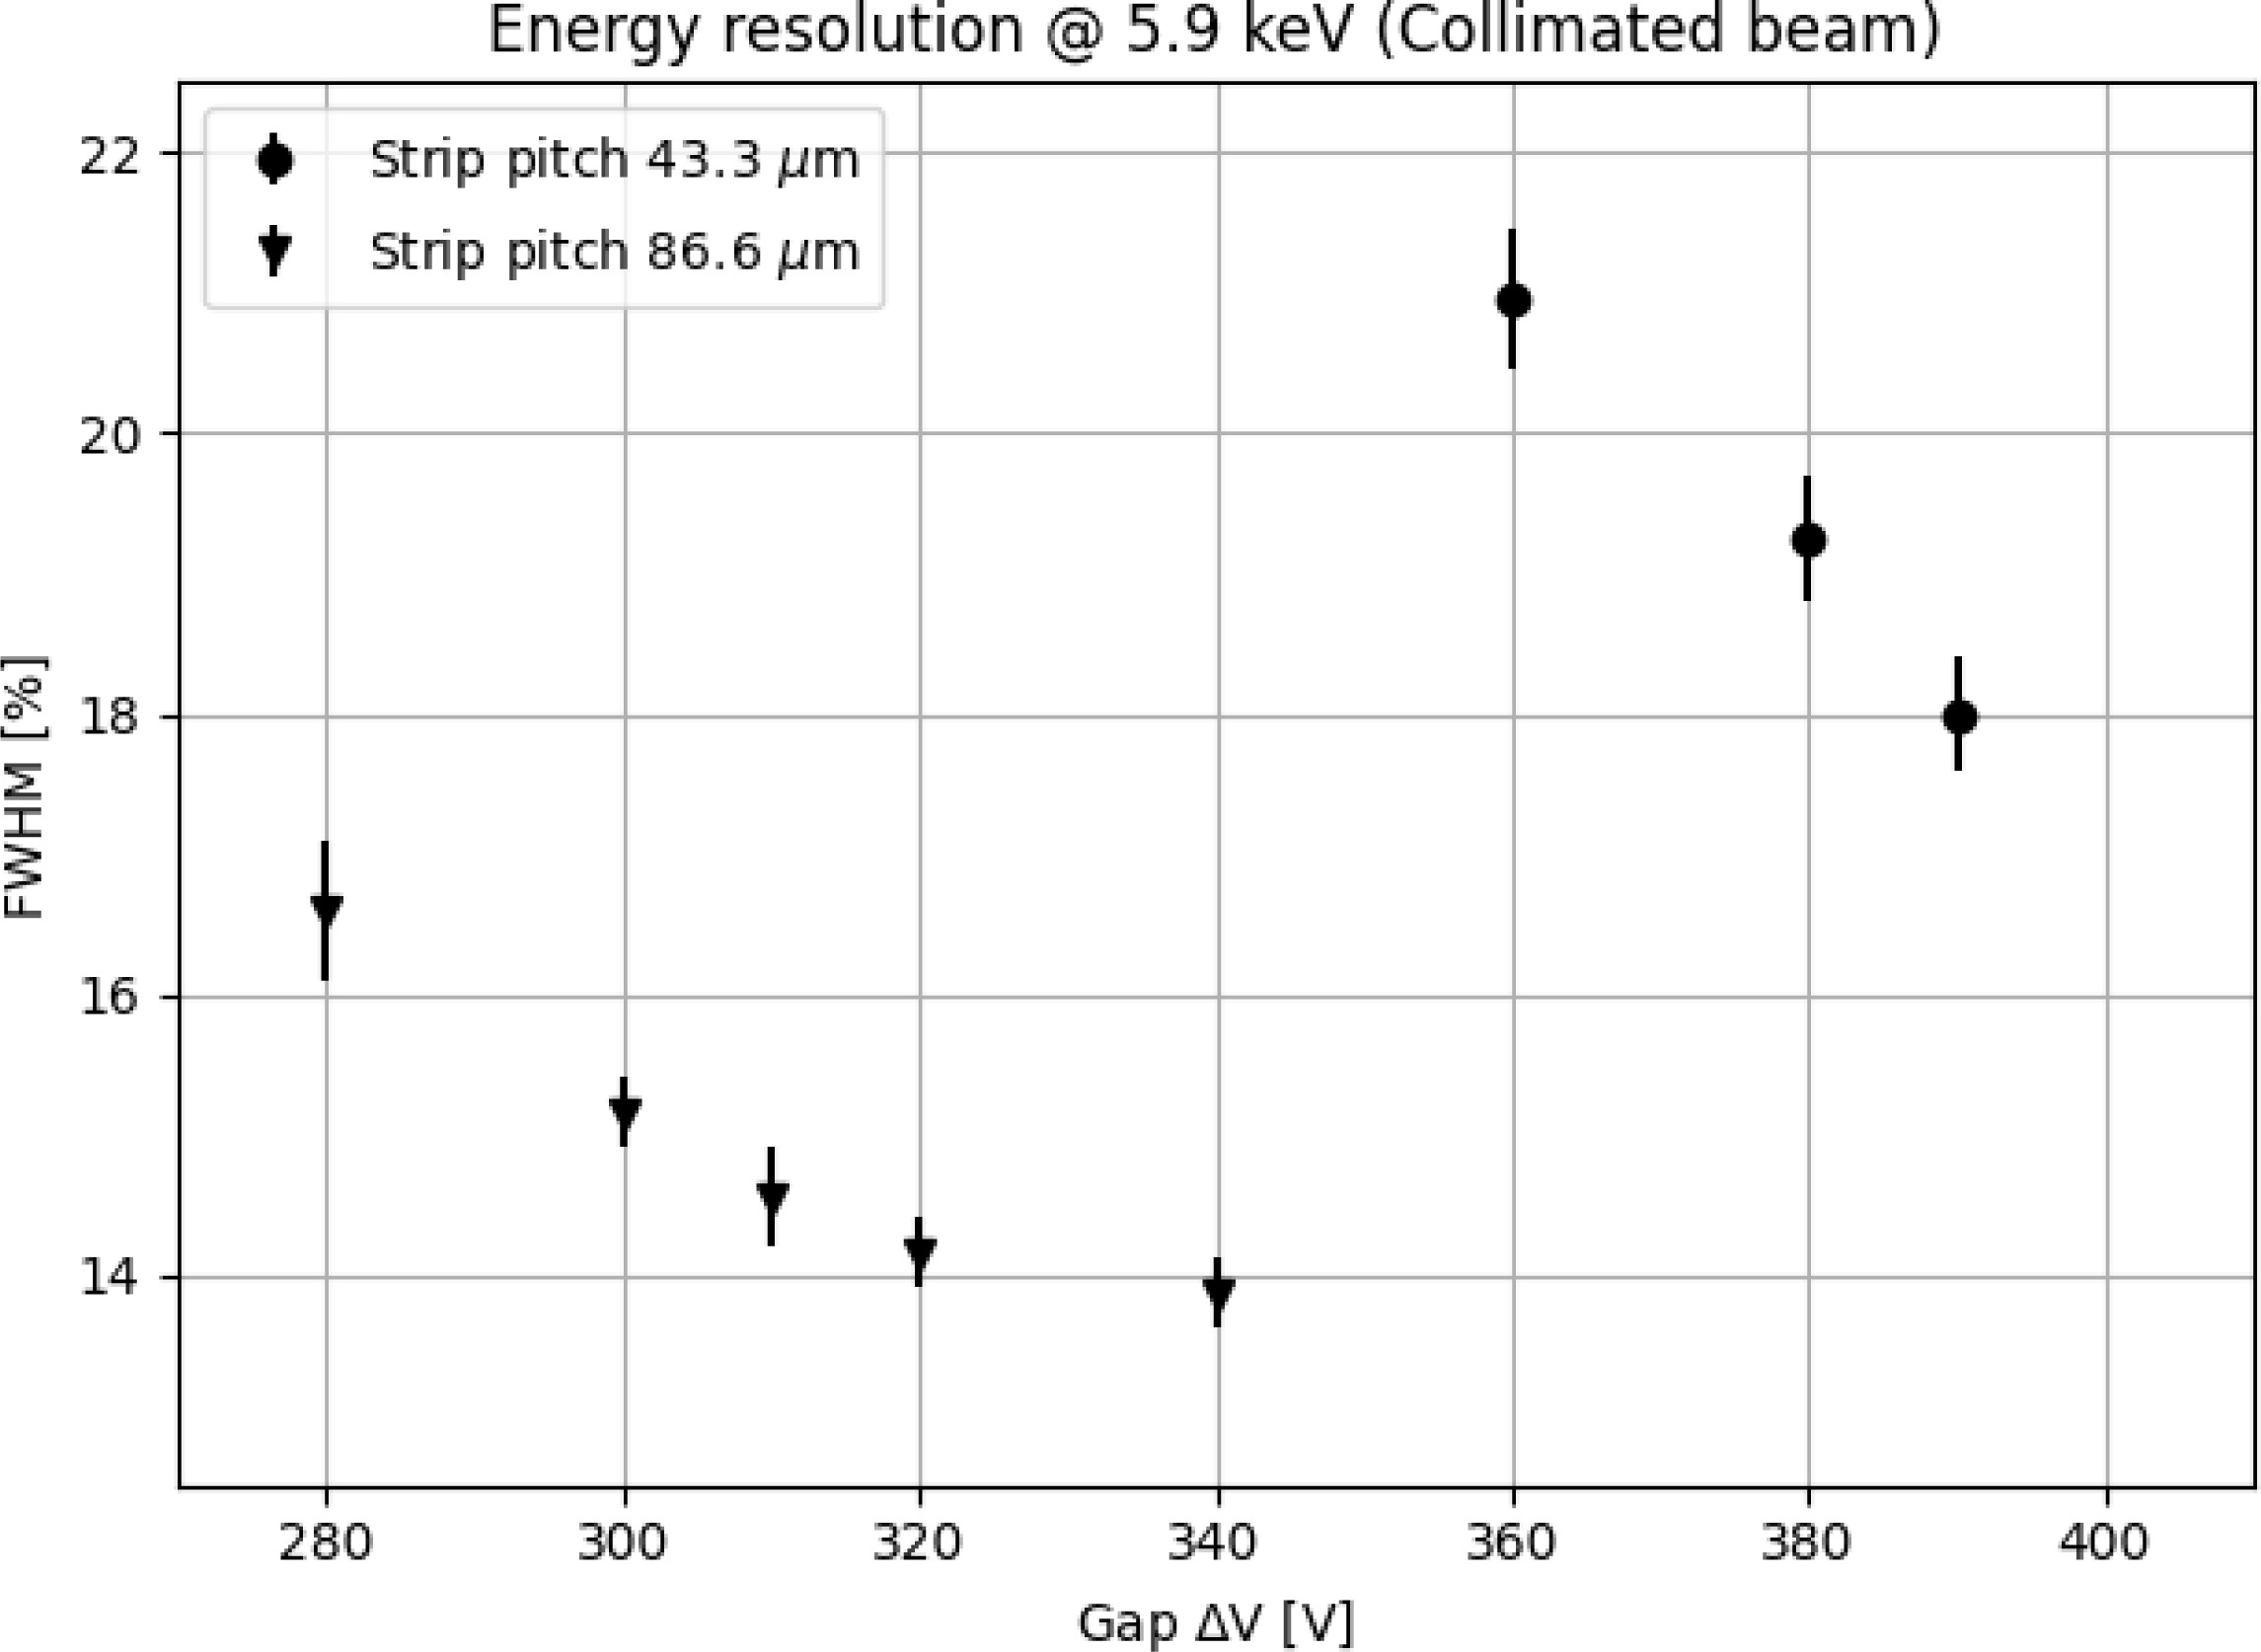
\includegraphics[width=0.49\linewidth]{figures/chapter5/resolution_wafer}
    \caption{Effective gain (left panel) and energy resolution (right panel) as a function of the anode-cathode voltage for one-dimensional structures with 43.3 $\mu$m and 86.6 $\mu$m pitch. Images taken from \cite{sgro2026}.}
    \label{fig:wafer_performance}
\end{figure}

These first results prove that these structures built directly and monolithically on top of a XPOL-like chip can operate as multiplication stage.


\subsection{Integration on XPOL ASICs}
After proving that the structures can work on top of a chip, the successive step is to test prototypes build directly on top of pre-existing chips to see if the expectations are confirmed.

The four designs described above are fabricated on top of an XPOL chip, dividing the active area into four different regions of $5 \times 5$ mm$^2$, one for each design. Fig. \ref{fig:mugpd_chip} shows a picture of a chip with the four different multiplication stages built on top of it. 

In this configuration the collection plane is represented by the pixels top metal electrode. An important thing that must be noted is that the current chips are designed to collect electrons, not ions, thus they are not able to read the signal produced by the avalanche generated by the micro-gaps.











